% =========================================================
% Required packages in the preamble:
% =========================================================
% \usepackage{booktabs}
% \usepackage{array}
% \usepackage{makecell}
% \usepackage{tabularx}
% \usepackage{float}
% \usepackage{placeins}

% =========================================================
% Appendix
% =========================================================

\clearpage
\onecolumn

\appendix
\section*{Appendix}
\addcontentsline{toc}{section}{Appendix}



\appendix
\section{Exploratory Overview of MSD Features}

\begin{figure}[H]
    \centering
    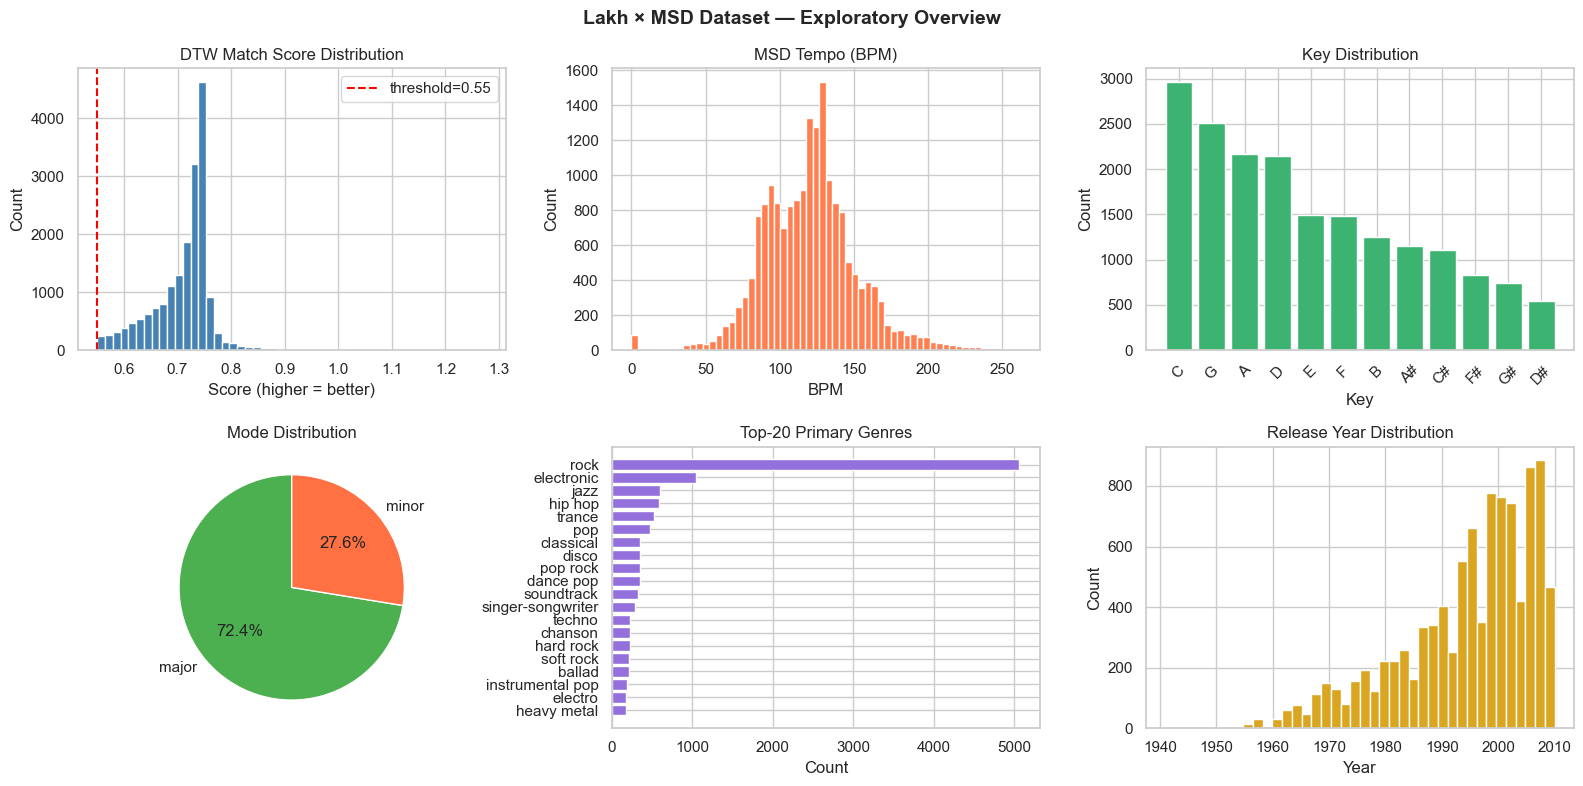
\includegraphics[width=0.99\linewidth]{sec/figures/output1.png}
    \caption{Exploratory Overview of MSD Features.}
    \label{fig:MSD_features}
\end{figure}

% =========================================================
\section{Exploratory Overview of User Taste Profile Filtering Pipeline and Features}


\begin{table}[H]
\centering
\caption{User dataset filtering pipeline statistics.}
\label{tab:data_filtering}
\begin{tabular}{l
                S[table-format=8.0]
                S[table-format=7.0]
                S[table-format=6.0]}
\toprule
\textbf{Step} &
\textbf{Interactions} &
\textbf{Unique Users} &
\textbf{Unique Songs} \\
\midrule
Raw            & 48373586 & 1019318 & 384546 \\
-- Mismatches  & 45795100 & 1019318 & 378309 \\
$\cap$ LMD     & 4243384  & 848243  & 7465   \\
-- Cold-start  & 3048959  & 299156  & 7227   \\
\bottomrule
\end{tabular}
\end{table}

\begin{figure}[H]
    \centering
    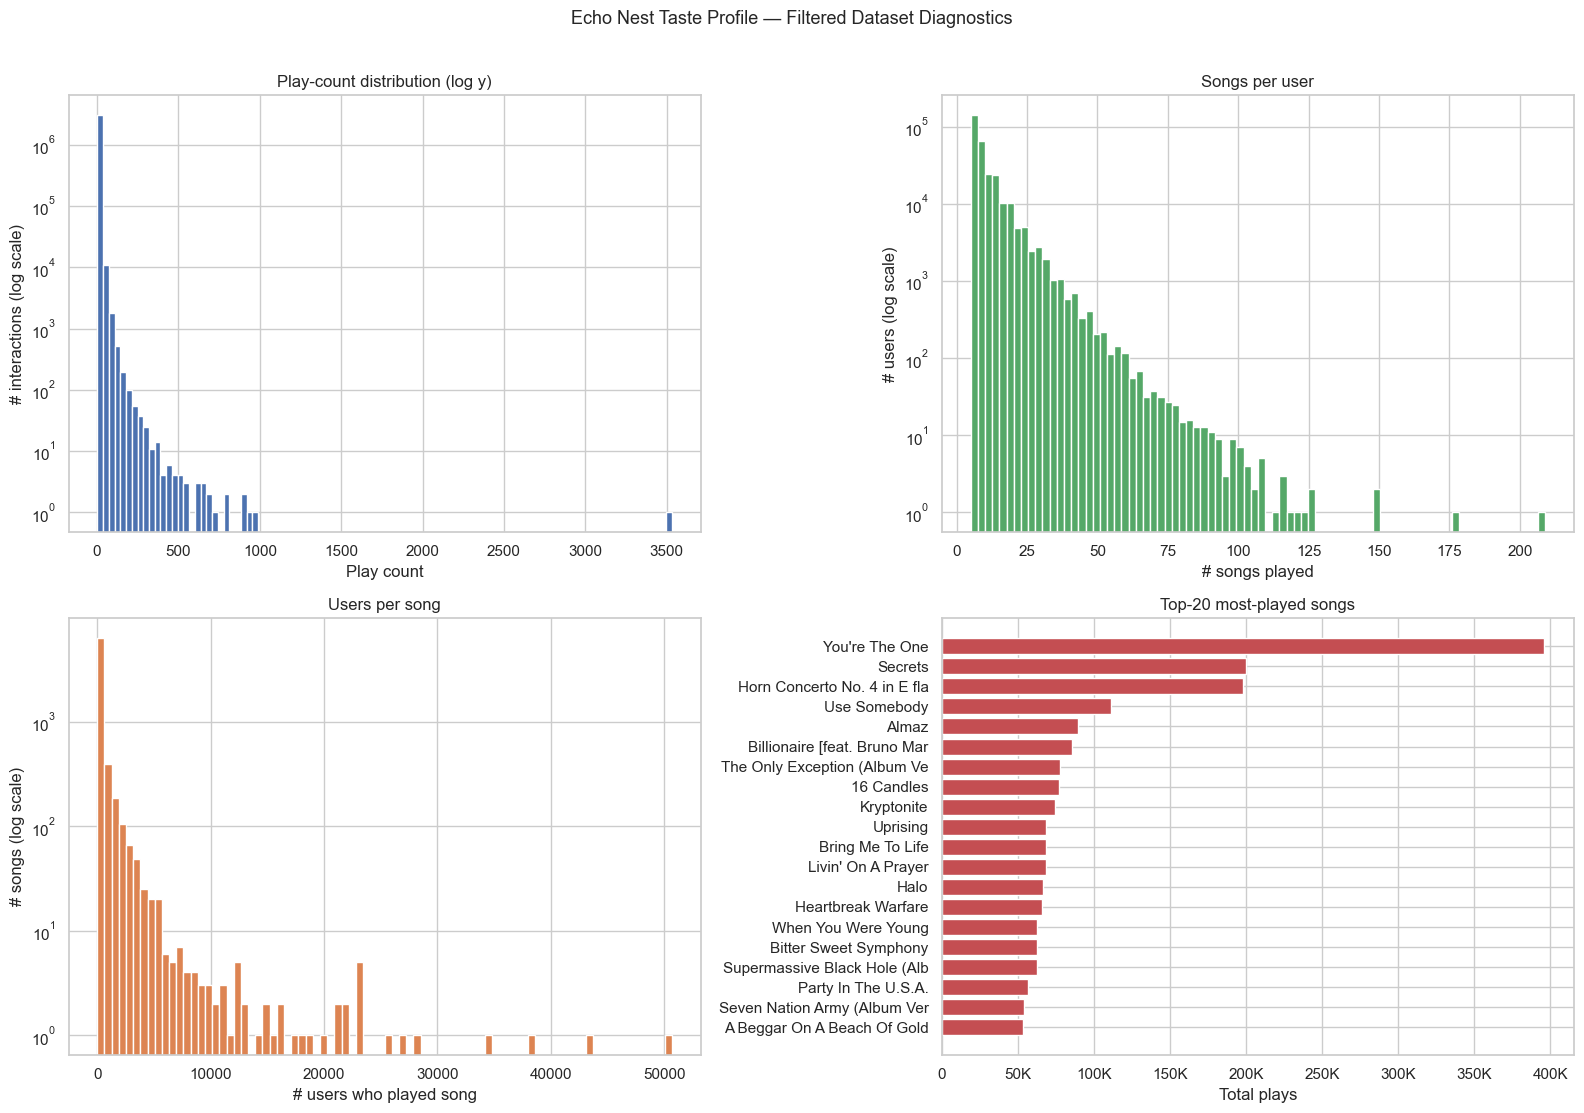
\includegraphics[width=0.99\linewidth]{sec/figures/user_diagnostics.png}
    \caption{Descriptive statistics of the filtered Echo Nest Taste Profile dataset, including the play-count distribution, songs per user, users per song, and the top-20 most-played songs.}
    \label{fig:user_diagnostics}
\end{figure}

% =========================================================
\section{Music-related feature inventory in simple knowledge graph}
% =========================================================
\footnotesize
\setlength{\tabcolsep}{3pt}
\renewcommand{\arraystretch}{1.15}
\begin{longtable}{
>{\ttfamily\bfseries\RaggedRight\arraybackslash}p{0.19\textwidth}
>{\RaggedRight\arraybackslash}p{0.31\textwidth}
>{\RaggedRight\arraybackslash}p{0.07\textwidth}
>{\ttfamily\RaggedRight\arraybackslash}p{0.23\textwidth}
>{\RaggedRight\arraybackslash}p{0.18\textwidth}
}
\caption{Music related MSD and jSymbolic features mapping to RDF representation}
\label{tab:kg_features}\\
\toprule
\textbf{Feature Name} &
\textbf{Description} &
\textbf{Origin} &
\textbf{RDF Term} &
\textbf{Storage Type} \\
\midrule
\endfirsthead
\toprule
\textbf{Feature Name} &
\textbf{Description} &
\textbf{Origin} &
\textbf{RDF Term} &
\textbf{Storage Type} \\
\midrule
\endhead
\bottomrule
\endfoot
track\_id &
Unique MSD track identifier used as the primary URI for the track node &
MSD &
mo:uuid (literal on track node) &
Literal (xsd:string)
\\
song\_id &
Echo Nest song identifier used for cross-referencing with Taste Profile &
MSD &
dct:identifier (literal on track node) &
Literal (xsd:string)
\\
artist\_id &
MSD canonical artist identifier used as the artist node URI &
MSD &
URI slug (artist namespace) &
Named Node (mo:Performer)
\\
artist\_mbid &
MusicBrainz cross-reference identifier for the artist &
MSD &
mo:musicbrainz\_guid &
Literal (xsd:string)
\\
artist\_name &
Display name of the artist &
MSD &
foaf:name &
Literal (xsd:string)
\\
title &
Title of the track &
MSD &
dct:title &
Literal (xsd:string)
\\
album\_name &
Name of the release/album the track belongs to &
MSD &
dct:isPartOf &
Literal (xsd:string)
\\
year &
Release year of the track &
MSD &
dct:date &
Literal (xsd:gYear)
\\
key &
Musical key of the track (C, C\#, D ... B) &
MSD &
mrc:hasKey &
Named Node (mrc:Key individual)
\\
mode &
Modality of the track (Major or Minor) &
MSD &
mrc:hasMode &
Named Node (mrc:Mode individual)
\\
loudness &
Overall loudness of the track in decibels &
MSD &
mrc:loudness &
Literal (xsd:double)
\\
primary\_genre &
Highest-weight genre tag of the artist; fallback weight 1.0 when no MSD weight available &
MSD &
mrc:hasGenre (via artist) &
Named Node (mrc:Genre individual)
\\
top3\_genres &
Top 3 genre tags of the artist with rank-based weights &
MSD &
mrc:hasGenre (via artist) &
Named Node (mrc:Genre individual)
\\
artist\_terms &
Full list of MSD genre/style tags with published weights &
MSD &
mrc:hasGenre (via artist) &
Named Node (mrc:Genre individual)
\\
midi\_instrument\_names &
List of General MIDI instrument names present in the MIDI file &
MIDI (LMD) &
mo:instrument (via performance) &
Named Node (mo:Instrument individual)
\\
tempo (Mean\_Tempo / msd\_tempo) &
Mean BPM of the track; jSymbolic value used when available, MSD scalar as fallback; stored on Performance and used to derive the categorical tempo class &
jSymbolic (MSD fallback) &
mo:tempo (via performance) &
Literal (xsd:double)
\\
Tempo class &
Categorical tempo marking derived from BPM (e.g. Allegro, Andante) &
Derived &
mrc:hasTempoClass (via performance) &
Named Node (mrc:TempoClass individual)
\\
Mean\_Tempo &
Mean tempo computed by jSymbolic &
jSymbolic &
mrc:meanTempo &
Literal (xsd:double)
\\
Initial\_Tempo &
Tempo at the start of the piece &
jSymbolic &
mrc:initialTempo &
Literal (xsd:double)
\\
Tempo\_Variability &
Variability of tempo across the piece &
jSymbolic &
mrc:tempoVariability &
Literal (xsd:double)
\\
Note\_Density &
Average number of notes per second &
jSymbolic &
mrc:noteDensity &
Literal (xsd:double)
\\
Average\_Note\_Duration &
Mean duration of individual notes &
jSymbolic &
mrc:averageNoteDuration &
Literal (xsd:double)
\\
Amount\_of\_Staccato &
Proportion of notes that are staccato &
jSymbolic &
mrc:amountOfStaccato &
Literal (xsd:double)
\\
Amount\_of\_Arpeggiation &
Degree of arpeggiated melodic motion &
jSymbolic &
mrc:amountOfArpeggiation &
Literal (xsd:double)
\\
Chromatic\_Motion &
Proportion of melodic intervals that are semitones &
jSymbolic &
mrc:chromaticMotion &
Literal (xsd:double)
\\
Chord\_Duration &
Mean duration of chords &
jSymbolic &
mrc:chordDuration &
Literal (xsd:double)
\\
\makecell[lt]{Average\_Number\_of\\_Independent\_ Voices} &
Mean number of simultaneous melodic voices &
jSymbolic &
\makecell[lt]{mrc:averageNumber\\OfIndependentVoices} &
Literal (xsd:double)
\\
\makecell[lt]{Average\_Note\_to\_Note\\_Change\_in\_Dynamics} &
Mean change in dynamics between consecutive notes &
jSymbolic &
\makecell[lt]{mrc:averageNoteTo\\NoteChangeIn\\Dynamics} &
Literal (xsd:double)
\\
\end{longtable}

% =========================================================
\section{User-related graph components}
% =========================================================

\begin{table}[H]
\centering
\caption{Taste Profile interaction features mapped to RDF representation.}
\label{tab:taste_profile_features}
\footnotesize
\setlength{\tabcolsep}{4pt}
\renewcommand{\arraystretch}{1.2}

\begin{tabular}{
>{\ttfamily\bfseries\raggedright\arraybackslash}p{3.0cm}
>{\raggedright\arraybackslash}p{4.8cm}
>{\raggedright\arraybackslash}p{1.6cm}
>{\ttfamily\raggedright\arraybackslash}p{4.0cm}
>{\raggedright\arraybackslash}p{3.2cm}
}
\toprule
\textbf{Feature Name} &
\textbf{Description} &
\textbf{Origin} &
\textbf{RDF Term} &
\textbf{Storage Type} \\
\midrule

user\_id &
Echo Nest user identifier used as the user node URI &
Echo Nest &
URI slug (user namespace) &
Named Node (mrc:Listener / foaf:Agent)
\\

play\_count &
Number of times a user played a track &
Echo Nest &
mrc:listenCount &
Literal (xsd:integer)
\\

user$\rightarrow$track interaction &
Listening interaction linking a user to a track &
Echo Nest &
\makecell[lt]{mrc:listenedTo (simple) /\\mrc:hasListeningInteraction\\(rich)} &
Edge (object property)
\\

\bottomrule
\end{tabular}
\end{table}

\section{Rich Knowledge Graph}
\begin{table}[!htbp]
\centering
\caption{Differences between the simple and rich knowledge graph representations.}
\label{tab:simple_vs_rich}
\footnotesize
\renewcommand{\arraystretch}{1.2}
\begin{tabular}{p{0.22\textwidth} p{0.30\textwidth} p{0.42\textwidth}}
\toprule
\textbf{Feature} & \textbf{Simple KG} & \textbf{Rich KG} \\
\midrule
Genre (\texttt{artist\_terms}, \texttt{primary\_genre}, \texttt{top3\_genres})
&
\begin{tabular}[t]{@{}l@{}}
Direct edge: \\
\texttt{artist} \\
\texttt{mrc:hasGenre} \\
\texttt{genre}
\end{tabular}
&
\begin{tabular}[t]{@{}l@{}}
Blank node: \\
\texttt{artist} \\
\texttt{mrc:hasGenreAssoc} \\
\texttt{[a mrc:GenreAssociation;} \\
\texttt{mrc:genre genre;} \\
\texttt{mrc:weight w]} \\
Direct edge retained
\end{tabular}
\\
\midrule
\texttt{artist\_terms\_weight}
&
Not stored
&
Stored as \texttt{mrc:weight} on the GenreAssociation blank node
\\
\midrule
\texttt{key}
&
Named node on Track (\texttt{mrc:hasKey})
&
Named node on Performance (\texttt{mrc:hasKey})
\\
\midrule
\texttt{mode}
&
Named node on Track (\texttt{mrc:hasMode})
&
Named node on Performance (\texttt{mrc:hasMode})
\\
\midrule
\texttt{key\_confidence}
&
Not stored
&
Stored as \texttt{mrc:keyConfidence} on Performance
\\
\midrule
\texttt{mode\_confidence}
&
Not stored
&
Stored as \texttt{mrc:modeConfidence} on Performance
\\
\midrule
\texttt{play\_count}
&
Not stored
&
Stored as \texttt{mrc:listenCount} on the ListeningEvent blank node
\\
\midrule
User$\rightarrow$Track interaction
&
\begin{tabular}[t]{@{}l@{}}
Direct edge: \\
\texttt{user} \\
\texttt{mrc:listenedTo} \\
\texttt{track}
\end{tabular}
&
\begin{tabular}[t]{@{}l@{}}
Blank node: \\
\texttt{user} \\
\texttt{mrc:hasListeningInteraction} \\
\texttt{[a mrc:ListeningEvent;} \\
\texttt{mrc:onTrack track;} \\
\texttt{mrc:listenCount n]}
\end{tabular}
\\
\bottomrule
\end{tabular}
\end{table}

\section{Knowledge Graph Inspection}
\begin{figure}[H]
    \centering
    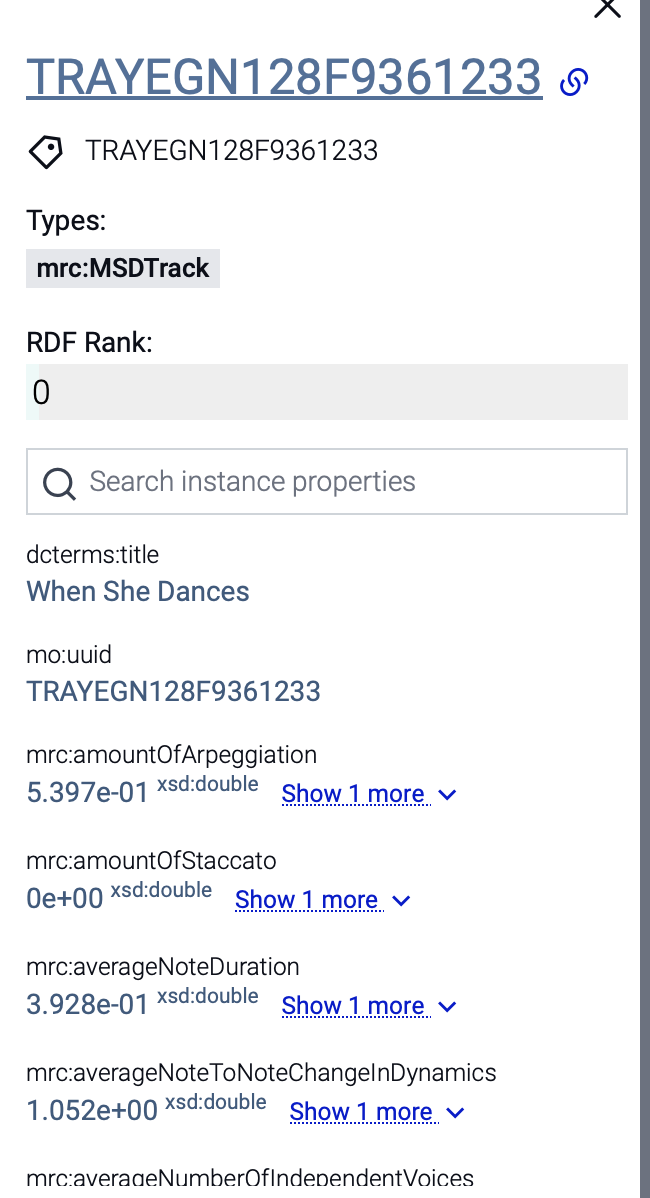
\includegraphics[width=0.75\linewidth]{sec/graph_DB/1.png}
    \caption{Selected properties of track node TRAYEGN128F9361233 (\textit{When She Dances}) as displayed in GraphDB, showing jSymbolic audio features and metadata stored directly on the \texttt{mrc:MSDTrack} instance.}
    \label{fig:1}
\end{figure}

\begin{figure}[H]
    \centering
    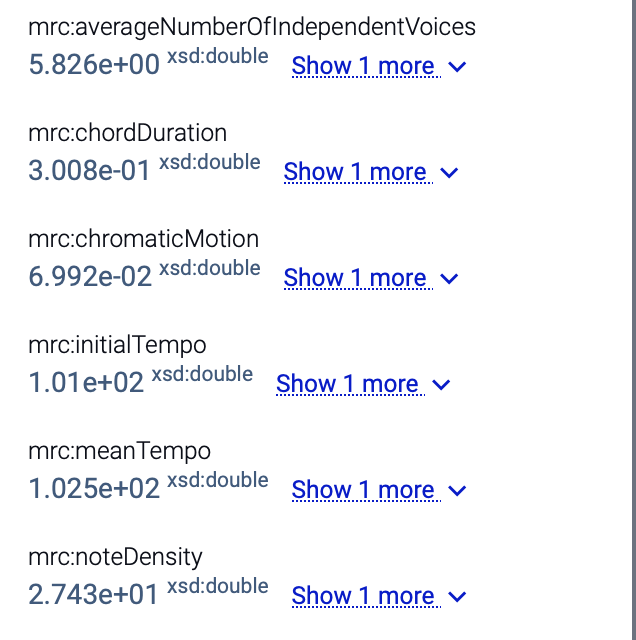
\includegraphics[width=0.75\linewidth]{sec/graph_DB/2.png}
    \caption{Selected properties of track node TRAYEGN128F9361233 (\textit{When She Dances}) as displayed in GraphDB, showing jSymbolic audio features and metadata stored directly on the \texttt{mrc:MSDTrack} instance.}
    \label{fig:2}
\end{figure}


\begin{figure}[H]
    \centering
    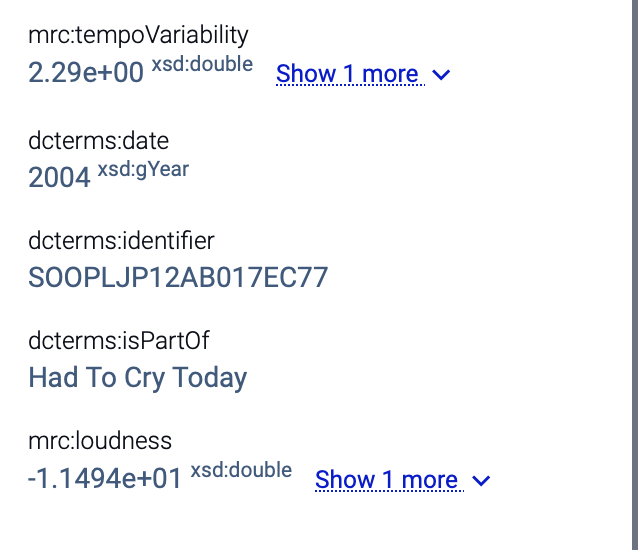
\includegraphics[width=0.75\linewidth]{sec/graph_DB/3.png}
    \caption{Selected properties of track node TRAYEGN128F9361233 (\textit{When She Dances}) as displayed in GraphDB, showing jSymbolic audio features and metadata stored directly on the \texttt{mrc:MSDTrack} instance.}
    \label{fig:3}
\end{figure}

% =========================================================
\clearpage
\section{SPARQL Query Examples and Results}
\label{sec:sparql_examples}
% =========================================================

All queries were executed against the knowledge graph loaded in GraphDB (or an equivalent in-memory rdflib graph for the simple KG). They share the following common prefix block, which is omitted from individual query listings for brevity:

\begin{footnotesize}
\begin{verbatim}
PREFIX mrc:   <http://purl.org/ontology/mrc/>
PREFIX mo:    <http://purl.org/ontology/mo/>
PREFIX rdfs:  <http://www.w3.org/2000/01/rdf-schema#>
PREFIX wdt:   <http://www.wikidata.org/prop/direct/>
PREFIX foaf:  <http://xmlns.com/foaf/0.1/>
PREFIX dct:   <http://purl.org/dc/terms/>
PREFIX owl:   <http://www.w3.org/2002/07/owl#>
\end{verbatim}
\end{footnotesize}

% ---------------------------------------------------------
\subsection*{Q1 — Genre Ranking, Simple KG}

Returns genres ranked by the number of distinct artists tagged with each genre. Direct \texttt{mrc:hasGenre} edges are used; no weights are stored in the simple KG.

\begin{footnotesize}
\begin{verbatim}
SELECT ?genreLabel (COUNT(DISTINCT ?artist) AS ?n_artists)
WHERE {
    ?artist mrc:hasGenre ?g .
    ?g      rdfs:label ?genreLabel .
    FILTER(LANG(?genreLabel) = "en")
}
GROUP BY ?genreLabel
ORDER BY DESC(?n_artists)
LIMIT 30
\end{verbatim}
\end{footnotesize}

\begin{table}[H]
\centering\footnotesize
\caption{Top 5 genres by artist count (Simple KG, truncated from 30 rows).}
\begin{tabular}{lr}
\toprule
Genre & \# Artists \\ \midrule
rock       & 2{,}117 \\
pop        & 1{,}062 \\
electronic & 1{,}037 \\
pop rock   &   814 \\
hip hop    &   381 \\
\bottomrule
\end{tabular}
\end{table}

% ---------------------------------------------------------
\subsection*{Q2 — Genre Ranking with Weights, Rich KG}

Uses the reified \texttt{mrc:GenreAssociation} blank nodes to aggregate per-artist tag weights, revealing salience differences hidden by raw artist counts.

\begin{footnotesize}
\begin{verbatim}
SELECT ?genreLabel
       (COUNT(DISTINCT ?artist)       AS ?n_artists)
       (ROUND(SUM(?w) * 1000) / 1000  AS ?total_weight)
       (ROUND(AVG(?w) * 1000) / 1000  AS ?avg_weight)
WHERE {
    ?artist mrc:hasGenreAssoc ?assoc .
    ?assoc  mrc:genre  ?g ;
            mrc:weight ?w .
    ?g      rdfs:label ?genreLabel .
    FILTER(LANG(?genreLabel) = "en")
}
GROUP BY ?genreLabel
ORDER BY DESC(?total_weight)
LIMIT 30
\end{verbatim}
\end{footnotesize}

\begin{table}[H]
\centering\footnotesize
\caption{Top 5 genres by aggregated weight (Rich KG). Note that \textit{electronic} overtakes \textit{pop} compared to Q1, reflecting stronger per-artist tagging.}
\begin{tabular}{lrrr}
\toprule
Genre & \# Artists & Total weight & Avg weight \\ \midrule
rock       & 2{,}117 & 1606.8 & 0.759 \\
electronic & 1{,}037 &  695.3 & 0.671 \\
pop        & 1{,}062 &  674.2 & 0.635 \\
pop rock   &   814   &  533.0 & 0.655 \\
hip hop    &   381   &  293.1 & 0.769 \\
\bottomrule
\end{tabular}
\end{table}

% ---------------------------------------------------------
\subsection*{Q3 — Track Key, Mode and Confidence (Rich KG)}

Retrieves the key, mode, tempo, and audio-analysis confidence scores for a specific track via the \texttt{mo:Performance} intermediate node. These confidence fields are only available in the rich KG.

\begin{footnotesize}
\begin{verbatim}
SELECT ?title ?keyLabel ?modeLabel ?keyConf ?modeConf ?tempo
WHERE {
    BIND(<http://purl.org/ontology/mrc/resource/track/TRBCNFO> AS ?t)
    ?t    dct:title      ?title .
    ?perf mrc:hasTrack   ?t ;
          mrc:hasKey     ?k ;
          mrc:hasMode    ?m .
    OPTIONAL { ?perf mo:tempo           ?tempo    }
    OPTIONAL { ?perf mrc:keyConfidence  ?keyConf  }
    OPTIONAL { ?perf mrc:modeConfidence ?modeConf }
    OPTIONAL { ?k rdfs:label ?keyLabel
               FILTER(LANG(?keyLabel) = "en") }
    OPTIONAL { ?m rdfs:label ?modeLabel
               FILTER(LANG(?modeLabel) = "en") }
}
\end{verbatim}
\end{footnotesize}

\noindent\textit{Example result} (track \textit{Into The Nightlife}):

\begin{table}[H]
\centering\footnotesize
\begin{tabular}{llllll}
\toprule
Title & Key & Mode & keyConf & modeConf & Tempo \\ \midrule
Into The Nightlife & A & Minor & 0.608 & 0.495 & 122.0 \\
\bottomrule
\end{tabular}
\end{table}

% ---------------------------------------------------------
\subsection*{Q4 — Artist Genre Weights via Blank Nodes (Rich KG)}

Demonstrates traversal of the reified \texttt{mrc:GenreAssociation} blank-node structure, returning genre labels and their MSD tag-strength weights for a specific artist.

\begin{footnotesize}
\begin{verbatim}
SELECT DISTINCT ?artistName ?genreLabel ?weight
WHERE {
    BIND(<http://purl.org/ontology/mrc/resource/artist/ARYM37E> AS ?a)
    ?a foaf:name         ?artistName ;
       mrc:hasGenreAssoc ?assoc .
    ?assoc  mrc:genre    ?g ;
            mrc:weight   ?weight .
    ?g      rdfs:label   ?genreLabel .
    FILTER(LANG(?genreLabel) = "en")
}
ORDER BY DESC(?weight)
\end{verbatim}
\end{footnotesize}

\noindent\textit{Example result} (artist \textit{Cyndi Lauper}):

\begin{table}[H]
\centering\footnotesize
\begin{tabular}{lll}
\toprule
Artist & Genre & Weight \\ \midrule
Cyndi Lauper & new wave   & 1.000 \\
Cyndi Lauper & ballad     & 0.673 \\
Cyndi Lauper & rock       & 0.600 \\
Cyndi Lauper & soundtrack & 0.525 \\
Cyndi Lauper & pop        & 0.300 \\
\bottomrule
\end{tabular}
\end{table}

% ---------------------------------------------------------
\subsection*{Q5 — Confidence-Filtered Key Distribution (Rich KG)}

Returns the distribution of musical keys restricted to performances where the audio analysis confidence is at least 0.8, filtering out unreliable key estimates.

\begin{footnotesize}
\begin{verbatim}
SELECT ?keyLabel (COUNT(*) AS ?n_high_confidence)
WHERE {
    ?perf a mo:Performance ;
          mrc:hasKey        ?k ;
          mrc:keyConfidence ?kc .
    FILTER(?kc >= 0.8)
    ?k rdfs:label ?keyLabel .
    FILTER(LANG(?keyLabel) = "en")
}
GROUP BY ?keyLabel
ORDER BY DESC(?n_high_confidence)
LIMIT 24
\end{verbatim}
\end{footnotesize}

\noindent The query returned 12 key labels. Top results: C\,(211), G\,(196), D\,(150), A\,(103), F\,(98), E\,(80)---consistent with the prevalence of these keys in Western popular music.

% ---------------------------------------------------------
\subsection*{Q6 — Decade Temporal Chain}

Verifies the temporal predecessor/successor structure of decade nodes and their alignment to parent century entities via Wikidata properties.

\begin{footnotesize}
\begin{verbatim}
SELECT ?prevLabel ?decadeLabel ?nextLabel ?centuryLabel
WHERE {
    ?decade a mrc:Decade ;
            rdfs:label ?decadeLabel .
    FILTER(LANG(?decadeLabel) = "en")
    OPTIONAL {
        ?decade rdfs:subClassOf ?century .
        OPTIONAL { ?century rdfs:label ?centuryLabel
                   FILTER(LANG(?centuryLabel) = "en") }
    }
    OPTIONAL {
        ?decade wdt:P155 ?prev .
        OPTIONAL { ?prev rdfs:label ?prevLabel
                   FILTER(LANG(?prevLabel) = "en") }
    }
    OPTIONAL {
        ?decade wdt:P156 ?next .
        OPTIONAL { ?next rdfs:label ?nextLabel
                   FILTER(LANG(?nextLabel) = "en") }
    }
}
ORDER BY ?decadeLabel
\end{verbatim}
\end{footnotesize}

\noindent\textit{Excerpt of results} (Wikidata IDs shown where English labels were not fetched):

\begin{table}[H]
\centering\footnotesize
\caption{Decade temporal chain results (selected rows).}
\begin{tabular}{llll}
\toprule
Prev & Decade & Next & Century \\ \midrule
---         & 1950s & 1960s & 20th century \\
1950s       & 1960s & 1970s & 20th century \\
1960s       & 1970s & 1980s & 20th century \\
1970s       & 1980s & 1990s & 20th century \\
1980s       & 1990s & 2000s & 20th century \\
1990s       & 2000s & 2010s & 21st century \\
2000s       & 2010s & ---   & 21st century \\
\bottomrule
\end{tabular}
\end{table}